\documentclass[11pt]{article}

\usepackage[utf8]{inputenc}
\usepackage[spanish]{babel}
\usepackage[margin=2.5cm]{geometry}
\usepackage{graphicx}
\usepackage{booktabs}
\usepackage{float}
\usepackage{hyperref}
\usepackage{amsmath}
\usepackage{caption}
\usepackage{subcaption}
\usepackage{enumitem}

\hypersetup{colorlinks=true, linkcolor=blue, urlcolor=blue, citecolor=blue}

\title{Tarea \#4: Pipeline Autónomo de Detección \\
Auto-etiquetado con Qwen VL, Transfer Learning y Validación \\
\large Reporte Técnico}
\author{
  Armando Rosas \and
  Alexandro Ruiz  \and
  José Camarillo \and
  Pedro Avila
}
\date{Agosto 2026}

\begin{document}

\maketitle
\tableofcontents
\newpage

% ============================================================
\section{Objetivo de la Tarea}
% ============================================================

El objetivo de este proyecto fue diseñar e implementar un pipeline de visión computacional
capaz de resolver el problema de escasez de datos etiquetados mediante el uso de un Modelo de
Lenguaje y Visión (VLM) de arquitectura abierta, \textbf{Qwen3.5}. El pipeline cubre cuatro
fases: (1) recolección y auto-etiquetado de 100 imágenes de perros husky mediante Qwen3.5, (2)
ajuste fino (\textit{transfer learning}) de un detector YOLOv8s sobre las anotaciones generadas
automáticamente, (3) un script de despliegue optimizado para inferencia, y (4) una etapa de
validación híbrida en cascada, donde cada detección de YOLOv8s es confirmada o descartada por
el mismo VLM en dos tamaños distintos (0.8B y 2B), permitiendo comparar el costo computacional
contra la mitigación de falsos positivos que aporta cada uno.

% ============================================================
\section{Metodología}
% ============================================================

\subsection{Fase 1: Recolección y auto-etiquetado con Qwen3.5}

Se recolectaron 100 imágenes de internet con múltiples instancias de perros husky por imagen.
Antes de procesarlas, se normalizó su nomenclatura al esquema \texttt{husky\_000.jpg}
\ldots\ \texttt{husky\_099.jpg} y se redujo el tamaño de cualquier imagen que excediera 1280px
en su lado más largo (20 de las 100 imágenes lo excedían), ya que algunas fotografías
originales alcanzaban resoluciones de hasta 5616$\times$3744px: el codificador visual de Qwen
convierte los píxeles de la imagen en ``tokens visuales'' cuyo costo de atención escala de
forma cuadrática, por lo que una imagen sobredimensionada puede requerir varios gigabytes de
memoria adicionales en una sola llamada de inferencia.

\paragraph{Selección del modelo.} Se utilizó Qwen3.5 en su versión \textbf{2B}
(\texttt{Qwen/Qwen3.5-2B}) para el etiquetado. La ejecución completa del pipeline final
(Fases~1 a~4, incluyendo el etiquetado con verificación de raza y el entrenamiento de YOLOv8s)
se realizó localmente en la siguiente laptop:

\begin{table}[H]
\centering
\caption{Especificaciones de hardware y software utilizadas}
\label{tab:specs}
\begin{tabular}{ll}
\toprule
\textbf{Componente} & \textbf{Especificación} \\
\midrule
Sistema operativo & Windows 10 \\
Procesador        & Intel Core i7-12650HX (12.\textsuperscript{a} generación) \\
RAM               & 16 GB \\
GPU               & NVIDIA GeForce RTX 4050 Laptop GPU \\
VRAM              & 6.0 GB \\
CUDA              & 12.1 \\
PyTorch           & 2.5.1+cu121 \\
Python            & 3.10.20 (conda-forge) \\
Ultralytics       & 8.4.95 \\
\bottomrule
\end{tabular}
\end{table}

\paragraph{Prompt de detección.} Se diseñó un prompt específico y estricto que pide
explícitamente \emph{todas} las instancias de husky visibles, cajas ajustadas sin adivinar
partes ocluidas, y una salida en formato JSON sin texto adicional:

\begin{quote}
\small\ttfamily
"Locate every single husky dog visible in this image, even if there are several of them. Do
not stop after the first one -- include ALL husky dogs you can see as separate entries in the
array. Output ONLY a JSON array, no explanation, no markdown fences, no bold/asterisks, in this
exact format: [\{"bbox\_2d": [x1, y1, x2, y2], "label": "husky dog"\}, ...] where coordinates
are normalized to a 0-1000 scale relative to the image width and height [...]"
\end{quote}

Esta versión sustituyó a un prompt inicial más breve, que en pruebas preliminares en ocasiones
se detenía tras detectar el primer perro de la imagen o variaba el formato de la salida (ver
análisis de sensibilidad, Sección~\ref{sec:cuestionario}).

\paragraph{Formato de salida de Qwen.} Aunque el prompt solicitaba inicialmente el orden
\texttt{[ymin, xmin, ymax, xmax]}, se verificó experimentalmente que Qwen3.5 responde de forma
consistente en su esquema nativo de \textit{grounding}
(\texttt{\{"bbox\_2d": [x1, y1, x2, y2], "label": ...\}}), en escala 0--1000. El prompt final se
ajustó para solicitar directamente ese formato nativo, y la conversión matemática al formato
YOLO (\texttt{class\_id x\_center y\_center width height}, normalizado 0--1) se implementó de
acuerdo a este orden de coordenadas. Adicionalmente, dado que Qwen3.5 puede operar en un modo
de razonamiento extendido que antepone un bloque de análisis interno a la respuesta, esta opción
se desactivó explícitamente para asegurar que la totalidad del presupuesto de tokens de
generación se destinara a la respuesta JSON esperada.

Cada imagen procesada generó un archivo \texttt{.txt} en formato YOLO y una visualización con
las cajas dibujadas para revisión manual. Las 100 imágenes fueron etiquetadas exitosamente.

\paragraph{Verificación de raza.} Para reducir la inclusión de perros de razas visualmente
similares al Husky Siberiano (notablemente el Alaskan Malamute) en las anotaciones automáticas,
se incorporó un segundo paso de verificación: cada caja detectada se recorta y se somete a una
consulta binaria adicional que confirma si la región corresponde específicamente a un Husky
Siberiano y no a otra raza ni a un lobo; las cajas no confirmadas se descartan antes de
escribirse. El mismo criterio estricto de exclusión de razas similares se incorporó también en
el prompt de detección inicial, como defensa complementaria, y en el prompt de validación
binaria de la Fase~4 (Sección~\ref{sec:fase4}).

\subsection{Fase 2: Transfer Learning de YOLOv8s}
\label{sec:fase2}

Las 100 imágenes etiquetadas se dividieron en un 70\,\% de entrenamiento (70 imágenes) y 30\,\%
de prueba (30 imágenes), con semilla fija para reproducibilidad, generando el archivo
\texttt{dataset.yaml} requerido por Ultralytics.

\paragraph{Augmentación de datos.} Dado el bajo volumen de datos, se configuró augmentación
agresiva: \texttt{mosaic=1.0}, \texttt{mixup=0.15}, \texttt{hsv\_h=0.015}, \texttt{hsv\_s=0.7},
\texttt{hsv\_v=0.4}, \texttt{fliplr=0.5}, \texttt{degrees=10.0}, \texttt{scale=0.5}.

\paragraph{Hiperparámetros de entrenamiento.} Para favorecer una convergencia estable dado el
bajo volumen de datos disponible (70 imágenes, 9 \textit{batches} por época), se utilizó el
optimizador AdamW con una tasa de aprendizaje de 0.0005, se congelaron las primeras 10 capas
correspondientes al \textit{backbone} preentrenado, y se permitieron hasta 60 épocas sin mejora
antes de detener el entrenamiento de forma anticipada.

\paragraph{Decisión de diseño: clase única, sin preservar clases de COCO.} El ajuste fino
estándar de Ultralytics con una sola clase de salida reinicializa la cabeza de detección,
perdiendo las 80 clases originales de COCO, incluso congelando el \textit{backbone}, ya que los
pesos de la red no son específicos por clase. Existe una técnica para preservar genuinamente las
clases originales (congelar las primeras 22 capas, entrenar una segunda cabeza de detección solo
para la clase nueva y fusionar ambas salidas), pero requiere modificar directamente la librería
de Ultralytics y se recomienda para conjuntos de 1000 o más imágenes de la clase nueva, muy por
encima de las 70 disponibles en este proyecto. Dado el alcance académico y el volumen de datos
disponible, se optó por el enfoque estándar de una sola clase; esta es una limitación deliberada
del pipeline, no un descuido.

\subsection{Fase 3: Despliegue del detector}

Se implementó un script de inferencia (\texttt{hybrid\_inference.py}) que carga los pesos
entrenados de YOLOv8s y procesa un flujo de imágenes midiendo latencia y FPS reales por imagen,
simulando un escenario de producción. Siguiendo la recomendación del enunciado de mantener un
umbral de confianza bajo para maximizar el número de detecciones que llegan a la etapa de
validación, el umbral de confianza del detector se fijó en 0.01, dejando que sea la cascada de
la Fase~4 la responsable de filtrar los falsos positivos, en lugar de descartarlos de forma
prematura en la etapa de detección.

\subsection{Fase 4: Validación híbrida en cascada}
\label{sec:fase4}

Cada detección de YOLOv8s se recorta, con un margen adicional de 10 píxeles alrededor de la
caja, y se envía a Qwen VL con un prompt binario de confirmación:

\begin{quote}
\small\ttfamily "Look only at this cropped image. Is the dog shown specifically a Siberian
Husky (not any other breed, and not a wolf)? Answer with exactly one word: Yes or No."
\end{quote}

Solo las detecciones cuya respuesta comienza con ``Yes'' se conservan; el resto se descarta
como falso positivo. Tras la cascada se aplica una segunda pasada de supresión de cajas
redundantes, necesaria porque el validador VLM confirma cada recorte de forma independiente,
sin considerar si otra caja ya aprobada cubre al mismo animal.

Siguiendo el requisito de comparación de la tarea, el pipeline se ejecutó de manera idéntica con
dos tamaños de validador, \textbf{Qwen3.5-0.8B} y \textbf{Qwen3.5-2B}, sobre el mismo equipo en
cada corrida (Tabla~\ref{tab:specs}), de forma que la comparación de latencia entre ambos sea
válida.

\subsection{Fase 5: Métricas}

Las métricas (mAP@0.5, precisión, \textit{recall}, falsos positivos/negativos, latencia y FPS)
se calculan mediante coincidencia de detecciones contra el \textit{ground truth} por IoU (umbral
0.5); el cómputo final del AP se realiza con la implementación de referencia de Ultralytics
(interpolación de 101 puntos, estilo COCO).

% ============================================================
\section{Resultados}
% ============================================================

\subsection{Tabla comparativa (conjunto de prueba, 30 imágenes / 60 cajas)}
\label{sec:tabla-test}

El conjunto de prueba corresponde al 30\,\% de las 100 imágenes originales que la Fase~2 nunca
usó para entrenar. El número de cajas de \textit{ground truth} (60) refleja el efecto del paso
de verificación de raza descrito en la Fase~1, que descarta anotaciones correspondientes a
razas visualmente similares al Husky Siberiano. Las tres configuraciones se evaluaron sobre el
mismo equipo de cómputo, por lo que la latencia y los FPS son directamente comparables entre
sí.

\begin{table}[H]
\centering
\small
\begin{tabular}{lccccccc}
\toprule
\textbf{Configuración} & \textbf{mAP@0.5} & \textbf{Precisión} & \textbf{Recall} &
\textbf{FP} & \textbf{FN} & \textbf{Latencia (ms)} & \textbf{FPS} \\
\midrule
YOLOv8s Ajustado (solo)          & 0.9350 & 0.4754 & 0.9667 & 64 & 2 & 23.41   & 42.72 \\
YOLOv8s + Qwen VL Validador (0.8B) & 0.9376 & 0.6706 & 0.9500 & 28 & 3 & 2198.84 & 0.45 \\
YOLOv8s + Qwen VL Validador (2B)   & 0.9549 & 0.6667 & 0.9667 & 29 & 2 & 2328.17 & 0.43 \\
\bottomrule
\end{tabular}
\caption{Comparativa de las 3 configuraciones del pipeline sobre el conjunto de prueba (60
cajas de \textit{ground truth} en 30 imágenes). FP/FN son conteos absolutos, no porcentajes.}
\label{tab:comparativa-test}
\end{table}

Con un umbral de confianza bajo, YOLOv8s solo genera un número considerable de detecciones de
baja confianza, y su precisión resulta baja en consecuencia (0.4754, 64 falsos positivos); esto
es esperado, dado que el umbral bajo existe justamente para que sea la cascada la que filtre, no
el detector. Ambos validadores cumplen ese rol de forma contundente, reduciendo los falsos
positivos de 64 a 28 y 29 respectivamente (más de la mitad), mientras el \textit{recall} se
mantiene prácticamente igual al del detector solo. El validador de 2B logra el mAP@0.5 más alto
de los tres (0.9549) y el menor número de falsos negativos (2, empatado con la línea base),
superando ligeramente al de 0.8B en precisión agregada; el de 0.8B tiene, a cambio, un falso
positivo menos (28 vs.\ 29). El costo de activar cualquiera de los dos validadores es una caída
de FPS de más de 90$\times$ frente al detector solo (Sección~\ref{sec:cuestionario}, pregunta
2).

\subsection{Curvas de entrenamiento (Fase 2)}

El entrenamiento corrió las 100 épocas completas sobre el conjunto de entrenamiento
re-etiquetado con verificación de raza, alcanzando mAP@0.5 $\approx 0.958$ y
mAP@0.5:0.95 $\approx 0.51$ sobre el conjunto de validación interno de Ultralytics (el mismo
conjunto de prueba de la Sección~\ref{sec:tabla-test}, usado también como \texttt{val} durante
el entrenamiento).

\begin{figure}[H]
\centering
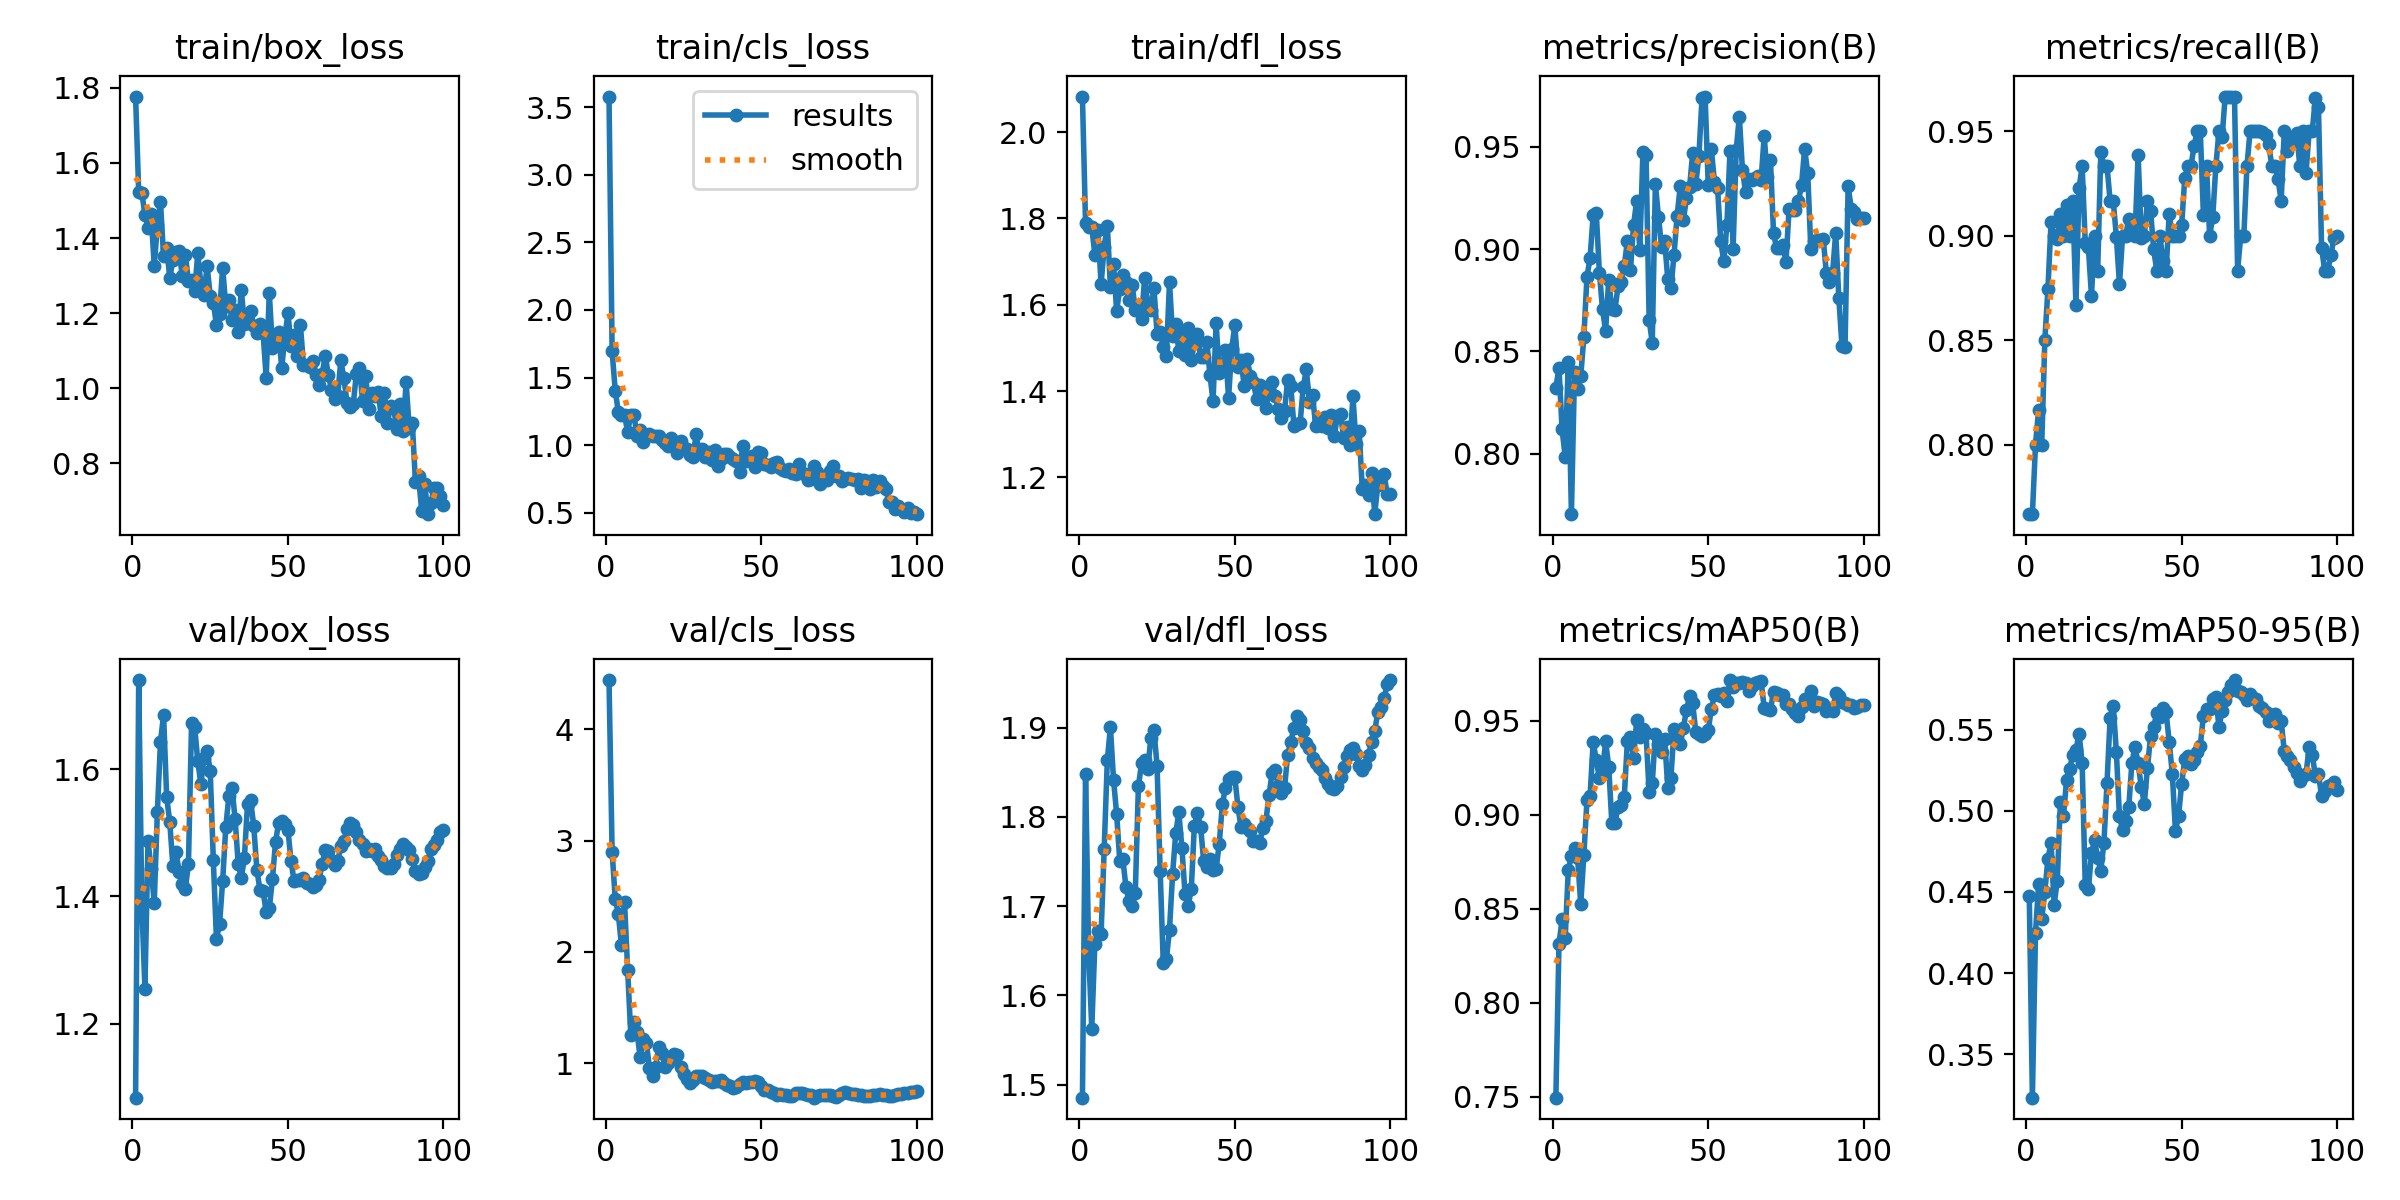
\includegraphics[width=0.95\textwidth]{../runs/detect/train/results.png}
\caption{Curvas de pérdida (\textit{box\_loss}, \textit{cls\_loss}, \textit{dfl\_loss}) y de
precisión/\textit{recall}/mAP@0.5 durante el entrenamiento.}
\label{fig:curvas-entrenamiento}
\end{figure}

\begin{figure}[H]
\centering
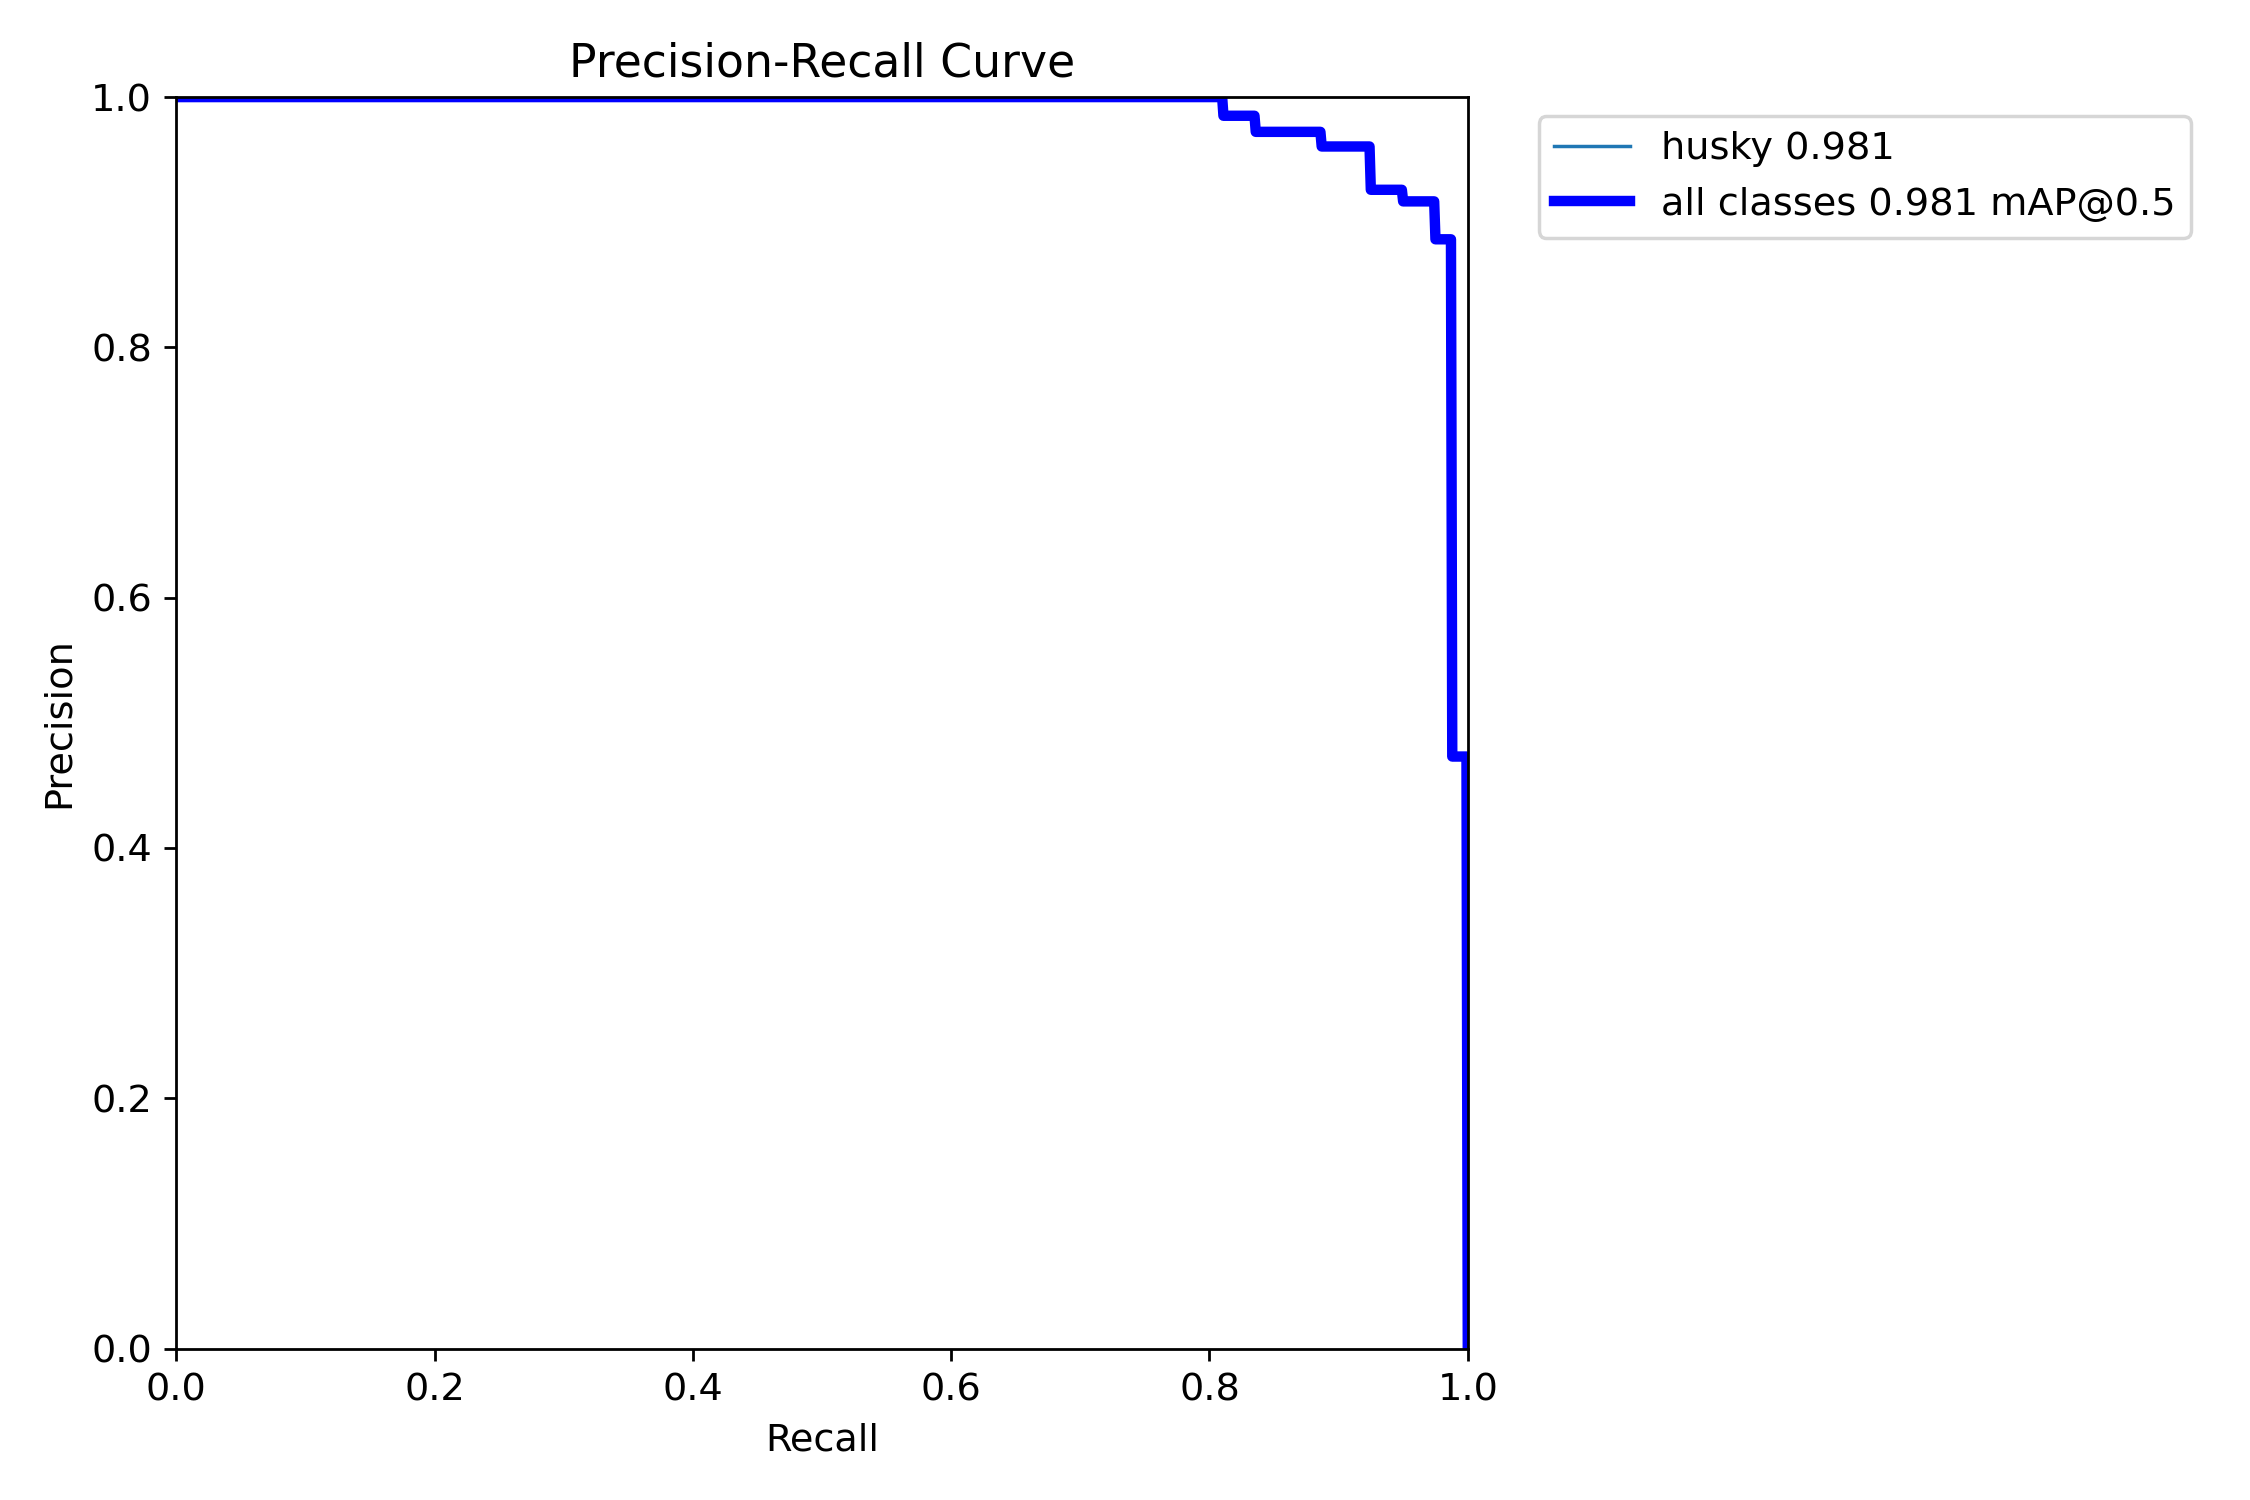
\includegraphics[width=0.7\textwidth]{../runs/detect/train/BoxPR_curve.png}
\caption{Curva Precision-Recall generada por Ultralytics sobre el conjunto de validación
interno al finalizar el entrenamiento.}
\label{fig:box-pr-entrenamiento}
\end{figure}

\subsection{Matriz de confusión (conjunto de prueba, 30 imágenes)}

\begin{figure}[H]
\centering
\begin{subfigure}{0.48\textwidth}
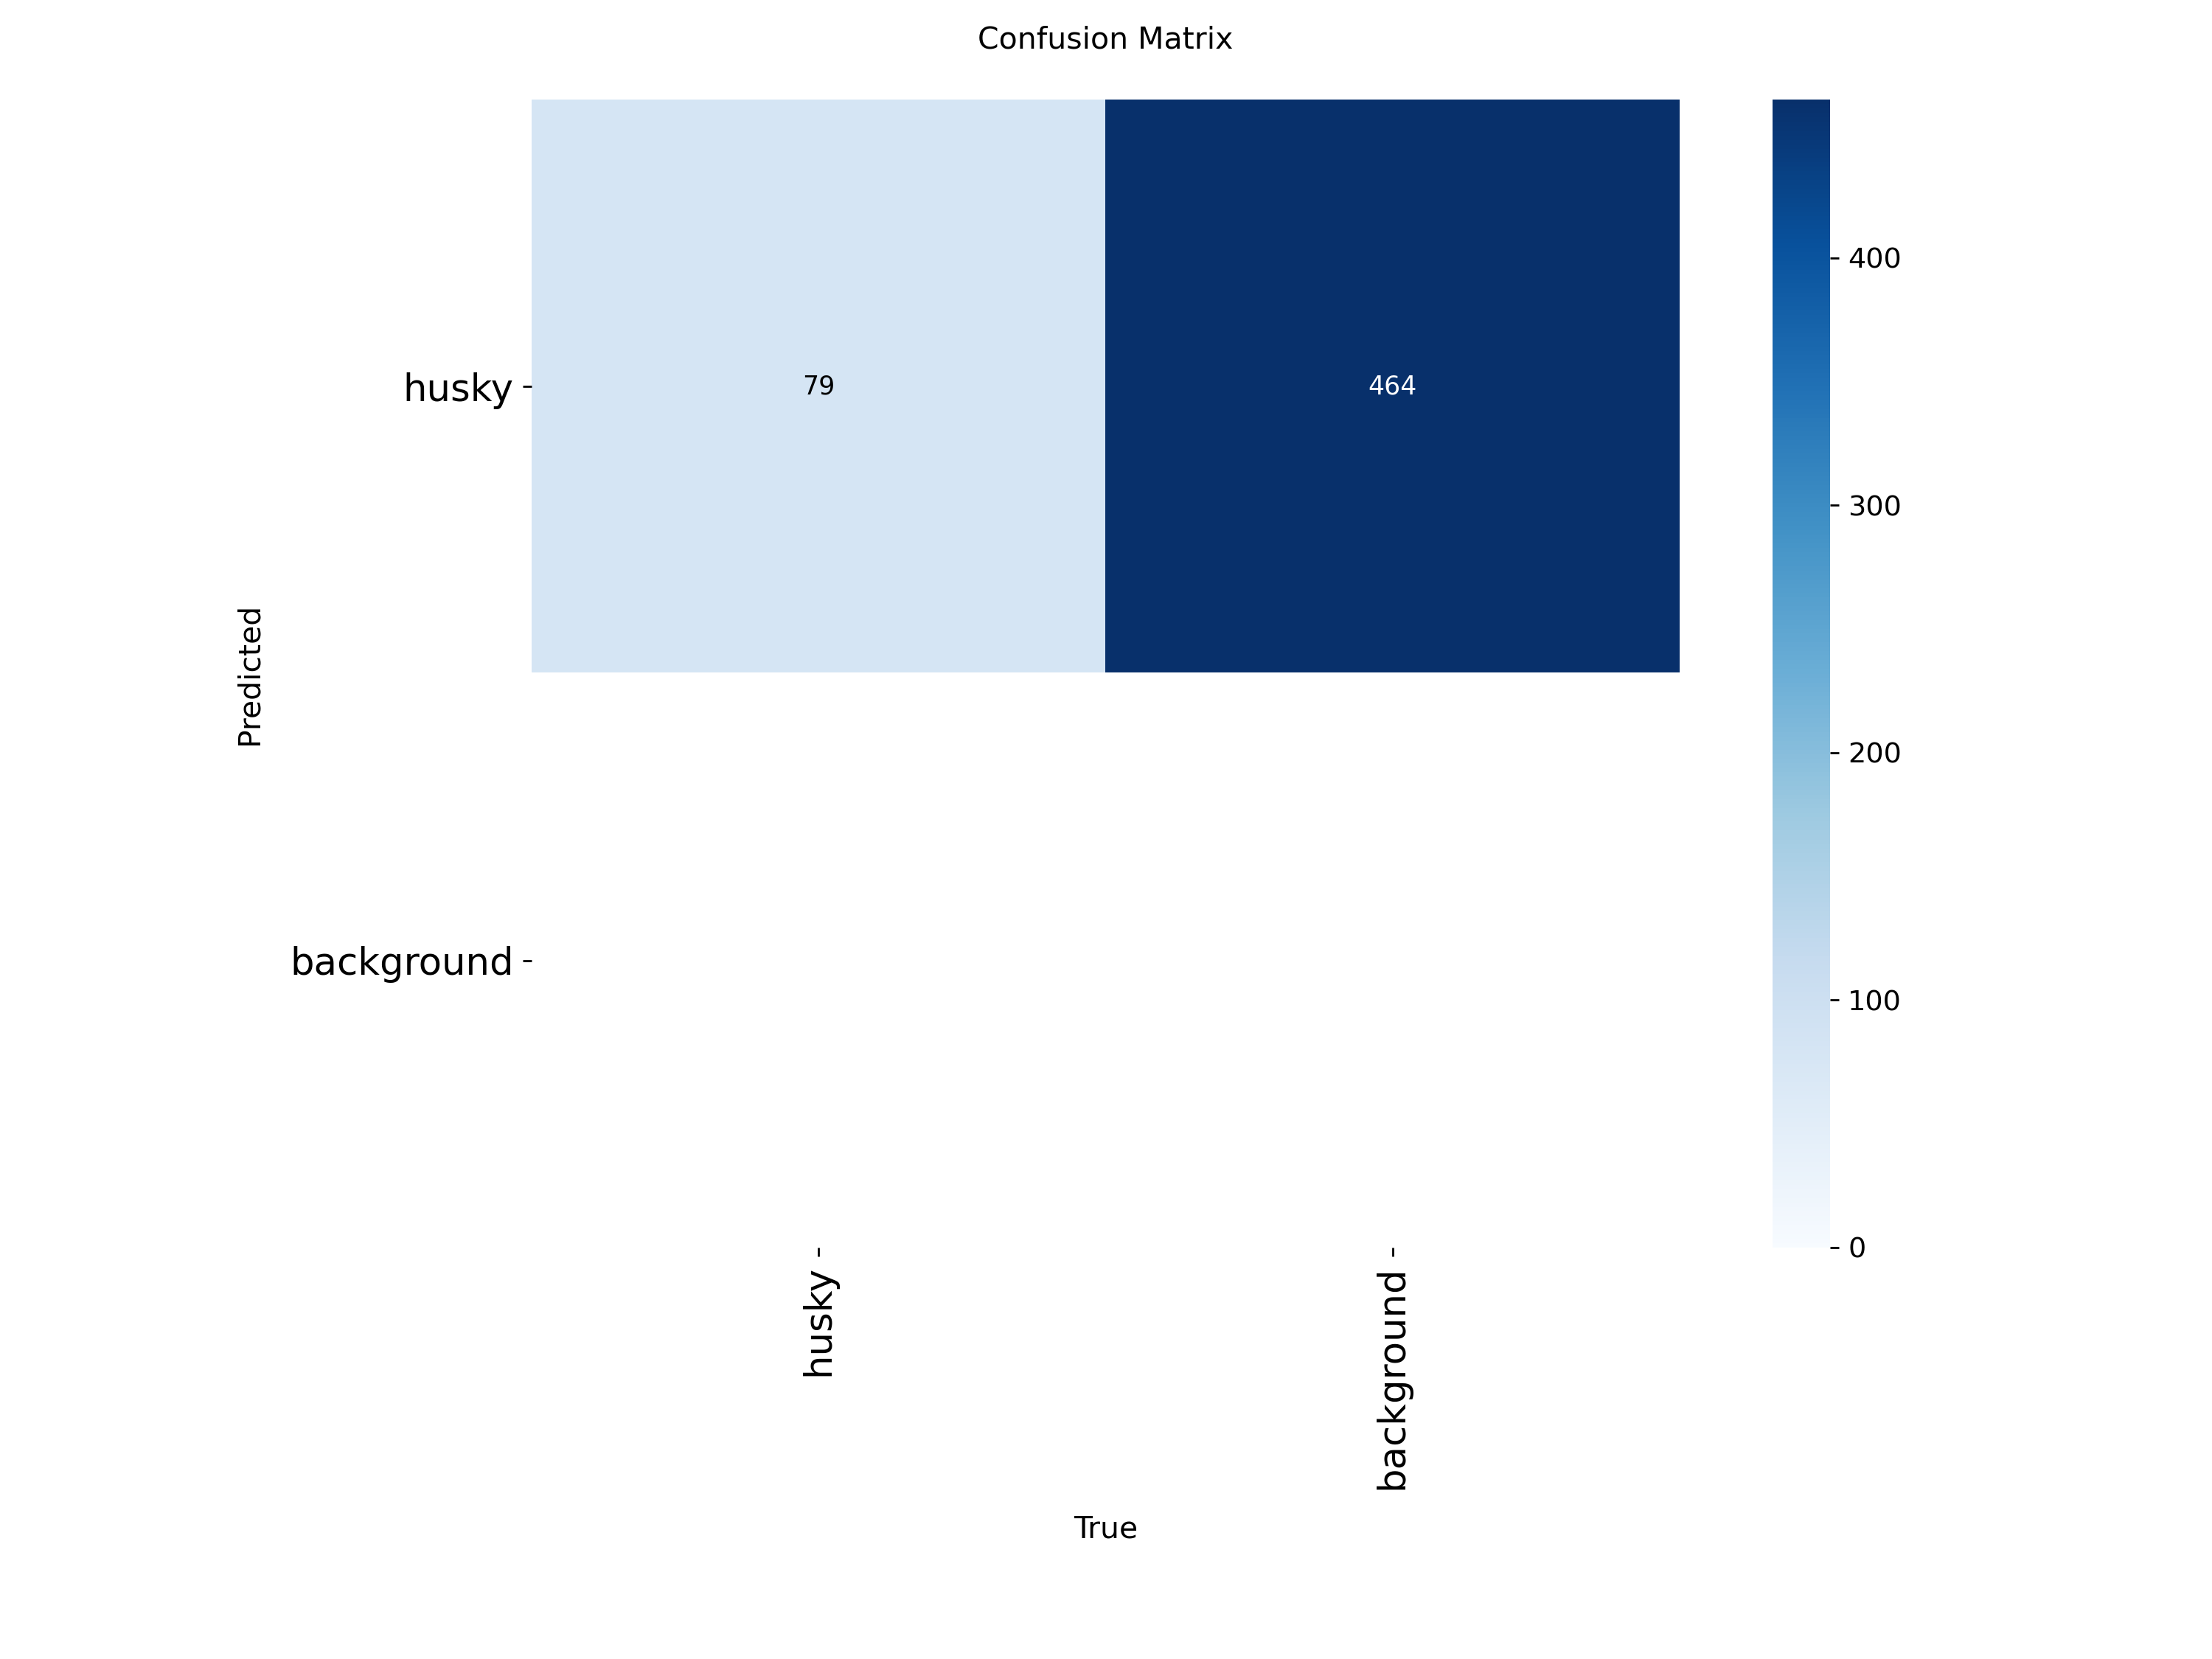
\includegraphics[width=\textwidth]{../runs/detect/train/confusion_matrix.png}
\caption{Absoluta}
\end{subfigure}
\hfill
\begin{subfigure}{0.48\textwidth}
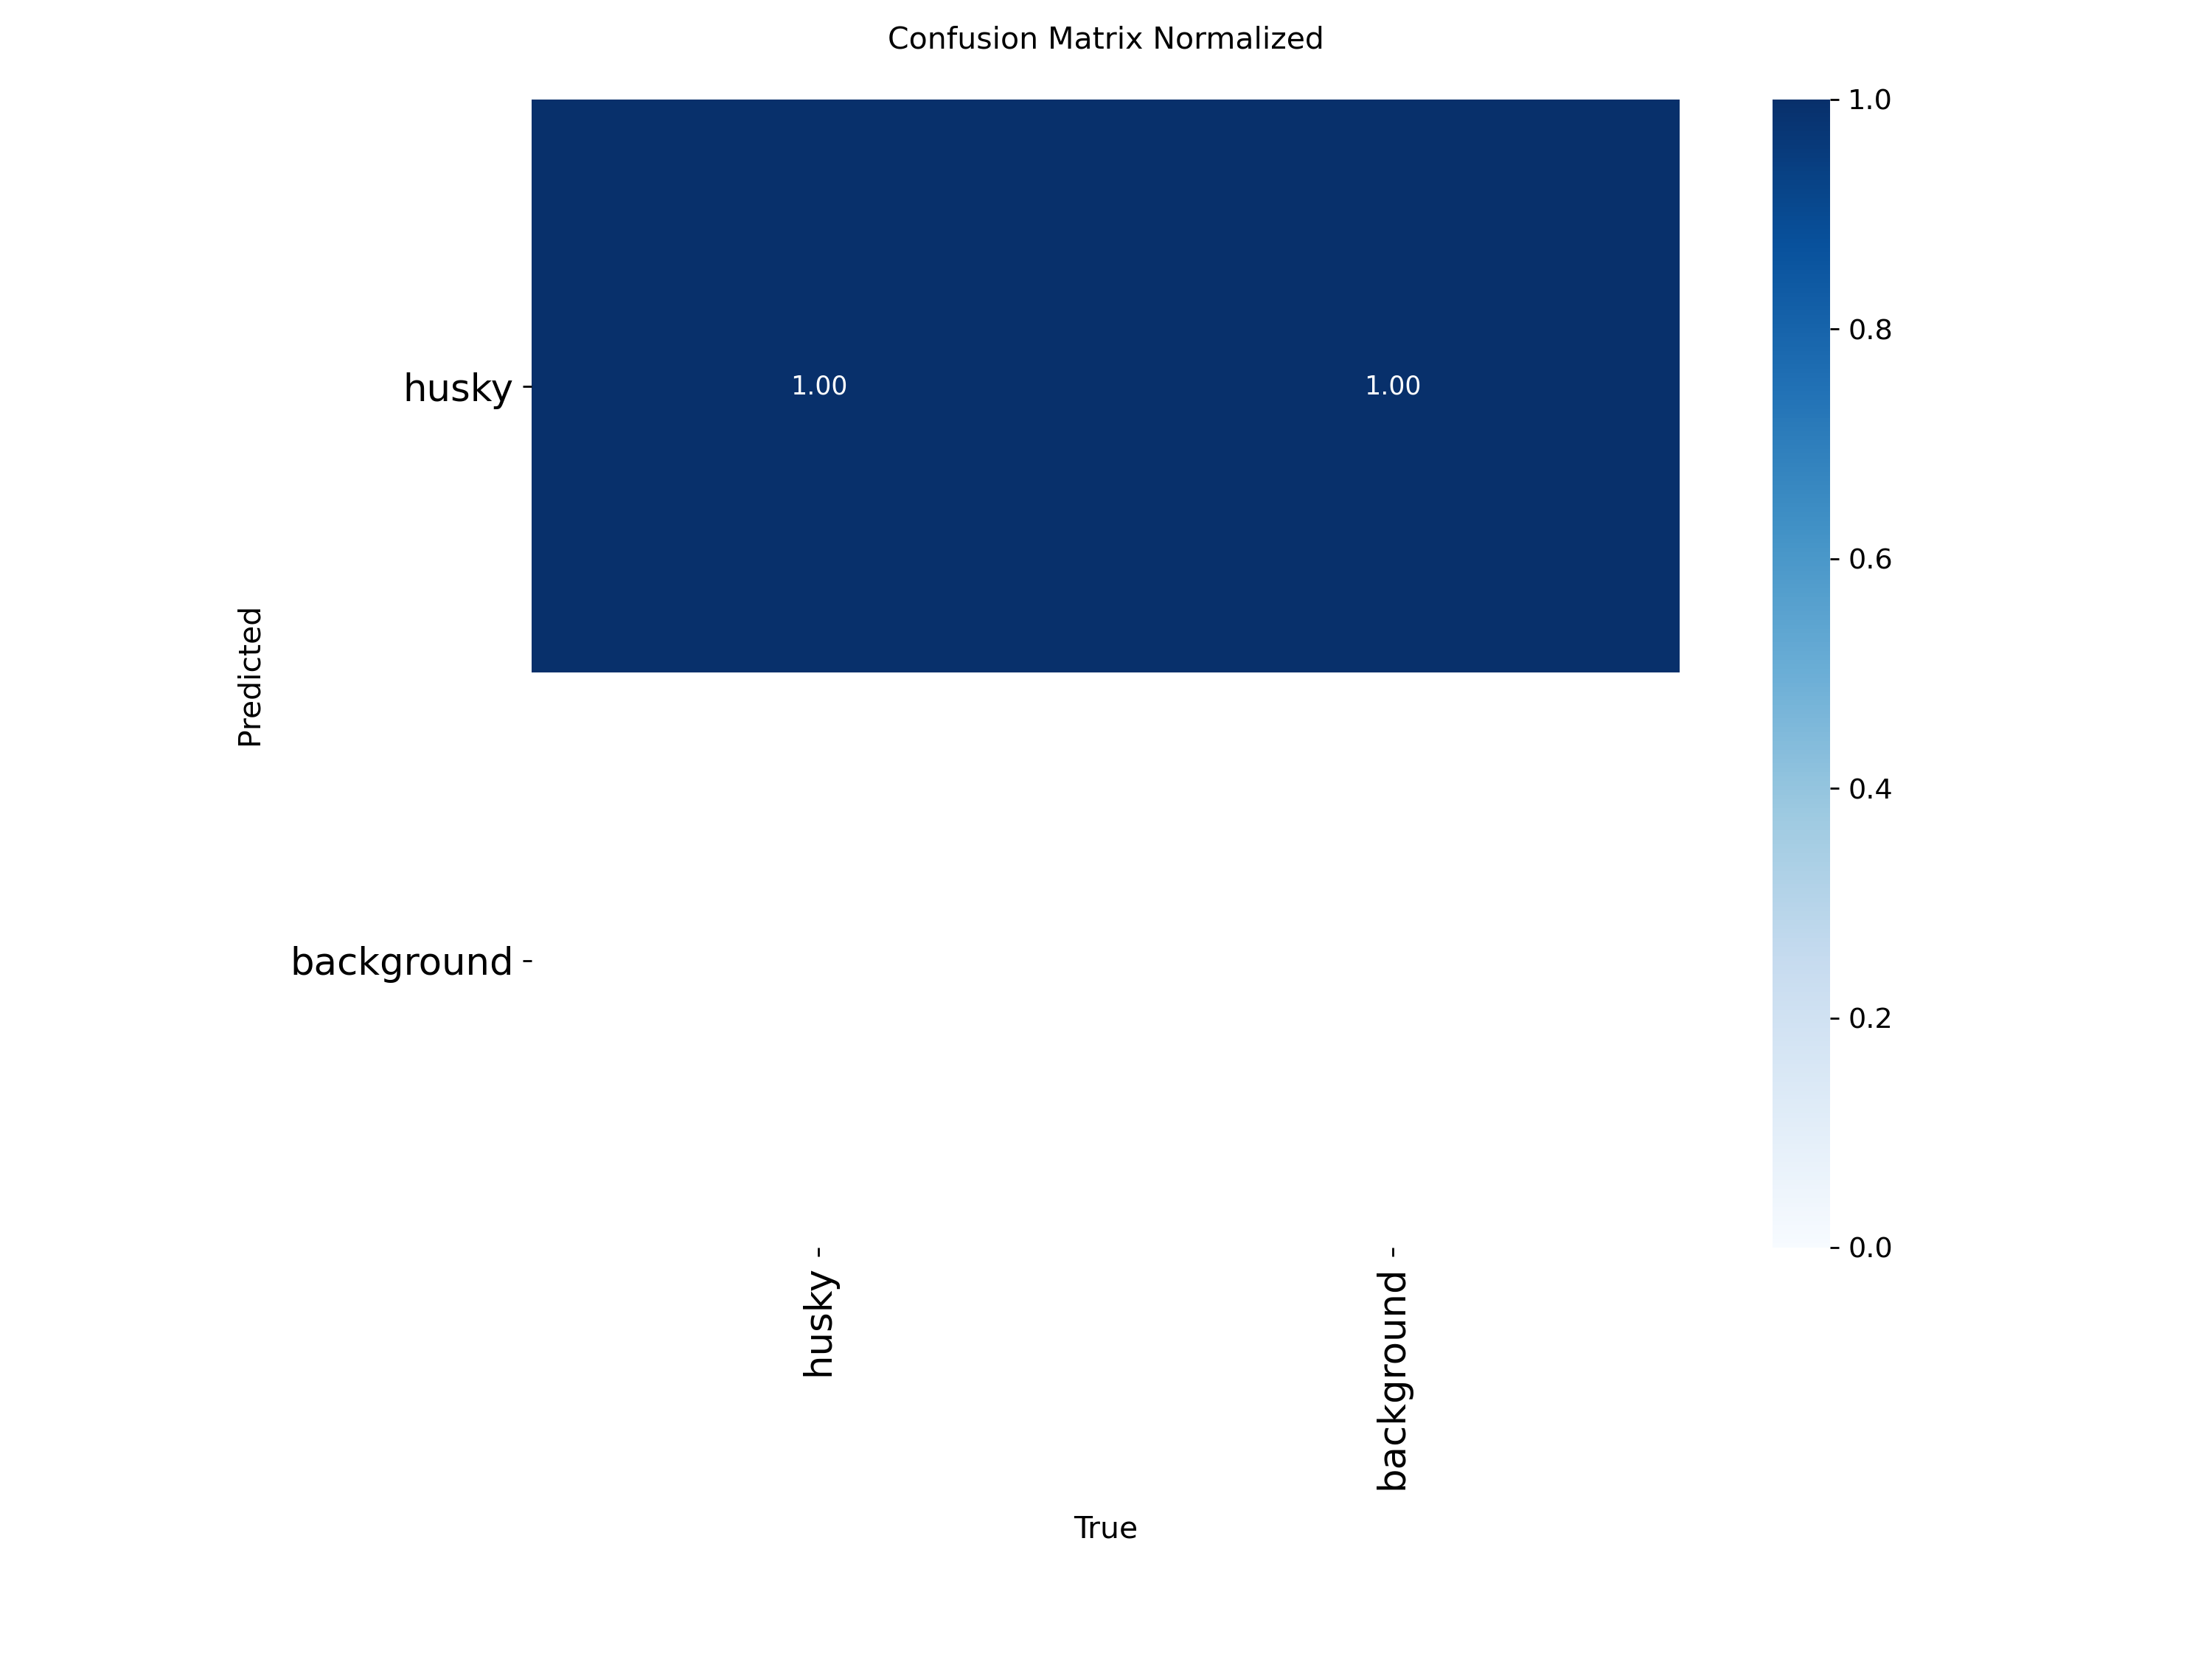
\includegraphics[width=\textwidth]{../runs/detect/train/confusion_matrix_normalized.png}
\caption{Normalizada}
\end{subfigure}
\caption{Matriz de confusión de YOLOv8s sobre el conjunto de prueba (30 imágenes), generada por
Ultralytics al finalizar el entrenamiento.}
\label{fig:matriz-confusion}
\end{figure}

\subsection{Curvas Precision-Recall @0.5 IoU (conjunto de prueba)}

\begin{figure}[H]
\centering
\begin{subfigure}{0.32\textwidth}
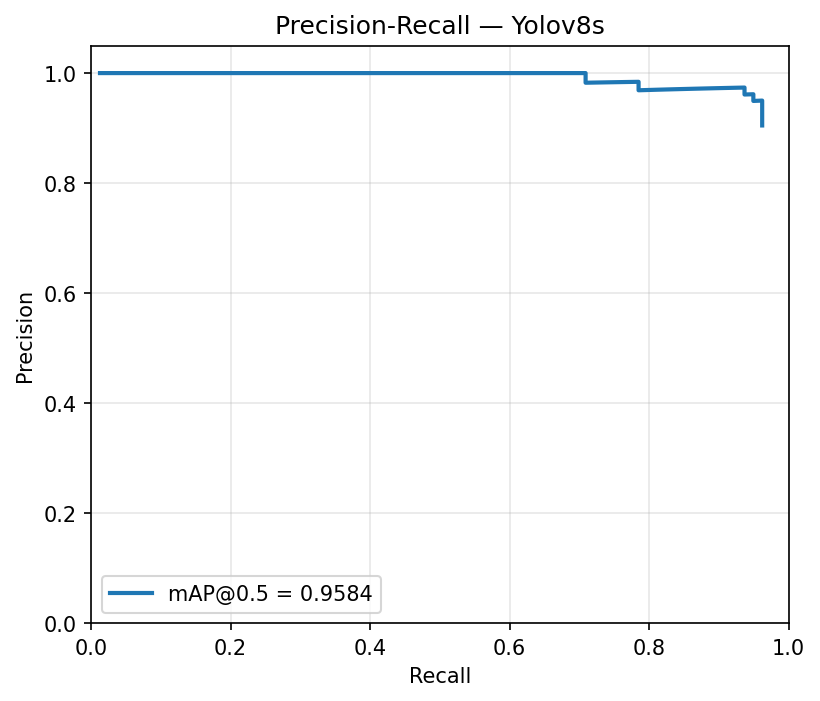
\includegraphics[width=\textwidth]{../results/graphs/Yolov8s_pr_curve.png}
\caption{YOLOv8s solo}
\end{subfigure}
\hfill
\begin{subfigure}{0.32\textwidth}
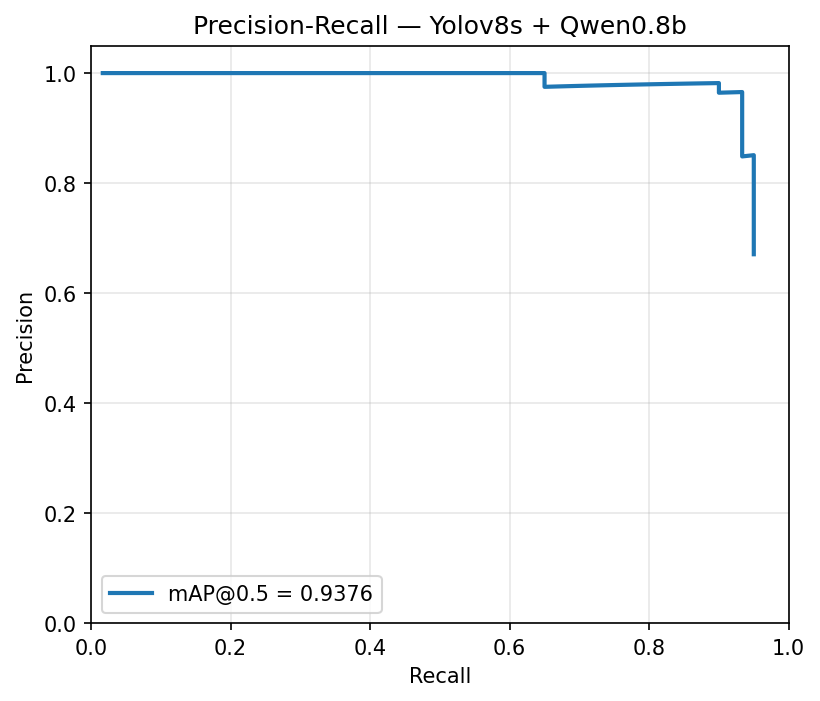
\includegraphics[width=\textwidth]{../results/graphs/Yolov8s + Qwen0.8b_pr_curve.png}
\caption{+ Qwen 0.8B}
\end{subfigure}
\hfill
\begin{subfigure}{0.32\textwidth}
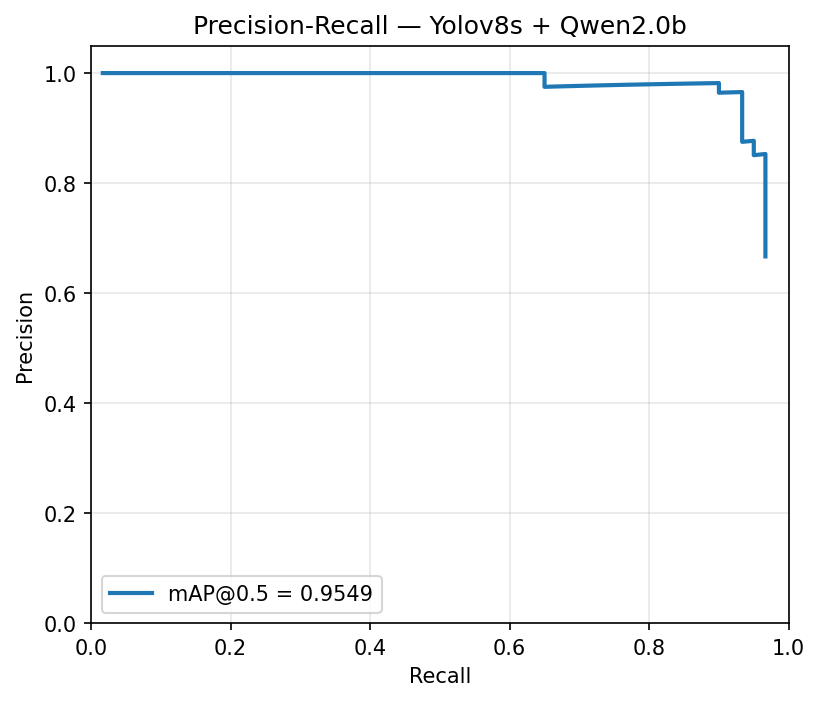
\includegraphics[width=\textwidth]{../results/graphs/Yolov8s + Qwen2.0b_pr_curve.png}
\caption{+ Qwen 2B}
\end{subfigure}
\caption{Curvas Precision-Recall individuales de las 3 configuraciones sobre el conjunto de
prueba.}
\label{fig:pr-individuales-test}
\end{figure}

\begin{figure}[H]
\centering
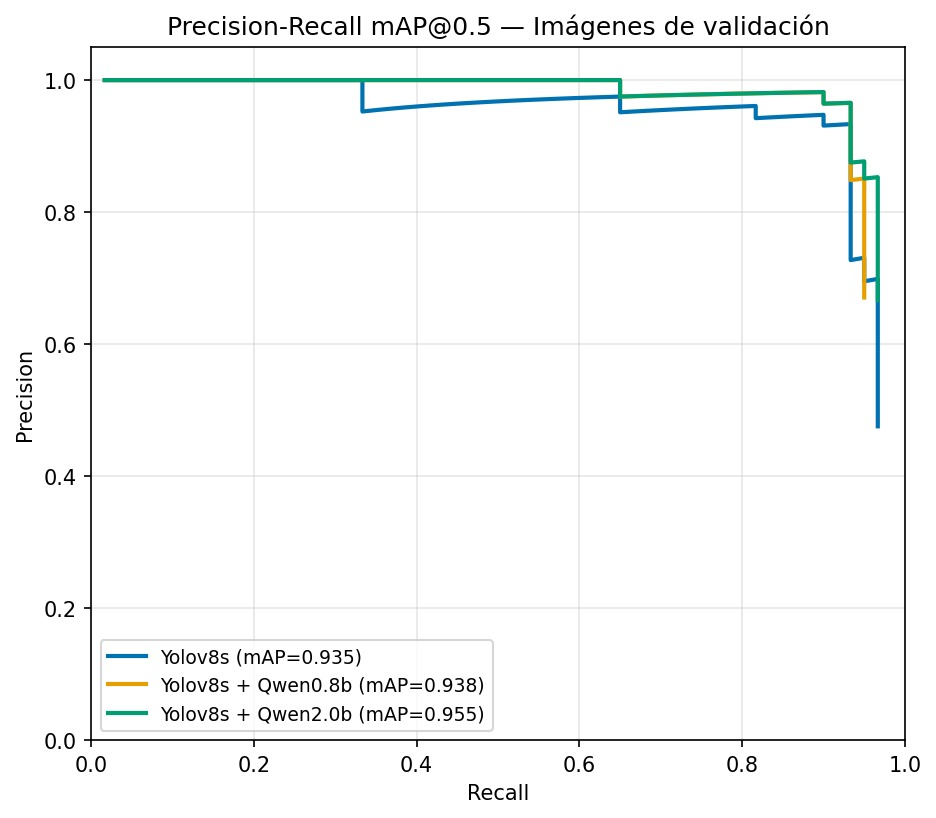
\includegraphics[width=0.75\textwidth]{../results/graphs/comparacion_pr_curves.jpeg}
\caption{Las 3 curvas Precision-Recall superpuestas para comparación directa (conjunto de
prueba).}
\label{fig:pr-comparacion-test}
\end{figure}
\clearpage

\subsection{Análisis de resultados visuales}

La Figura~\ref{fig:ejemplos-cascada} muestra la misma imagen del conjunto de prueba procesada
por las 3 configuraciones: las cajas verdes son verdaderos positivos (coinciden con
\textit{ground truth}) y las naranjas son falsos positivos. Se observa cómo la cascada de
validación reduce las cajas naranjas frente al detector solo.

\begin{figure}[H]
\centering
\begin{subfigure}{0.32\textwidth}
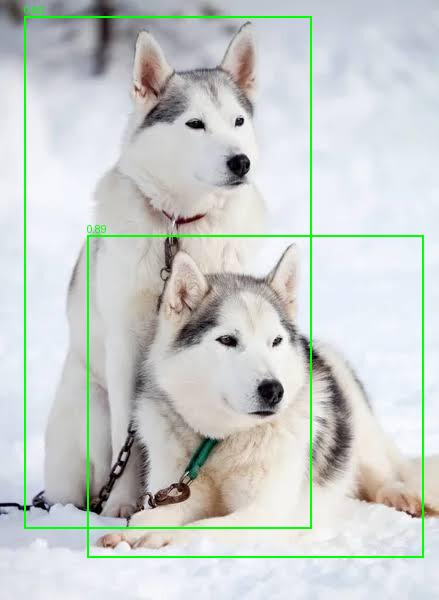
\includegraphics[width=\textwidth]{../results/figures/Yolov8s/husky_000.jpg}
\caption{YOLOv8s solo}
\end{subfigure}
\hfill
\begin{subfigure}{0.32\textwidth}
\includegraphics[width=\textwidth]{../results/figures/Yolov8s + Qwen0.8b/husky_000.jpg}
\caption{+ Qwen 0.8B}
\end{subfigure}
\hfill
\begin{subfigure}{0.32\textwidth}
\includegraphics[width=\textwidth]{../results/figures/Yolov8s + Qwen2.0b/husky_000.jpg}
\caption{+ Qwen 2B}
\end{subfigure}
\caption{\texttt{husky\_000.jpg} (conjunto de prueba) procesada por las 3 configuraciones.
Verde = verdadero positivo, naranja = falso positivo.}
\label{fig:ejemplos-cascada}
\end{figure}

Las Figuras~\ref{fig:exito}--\ref{fig:falla} complementan el ejemplo anterior con tres casos
elegidos para ilustrar cada categoría requerida por el análisis.

\begin{figure}[H]
\centering
\begin{subfigure}{0.32\textwidth}
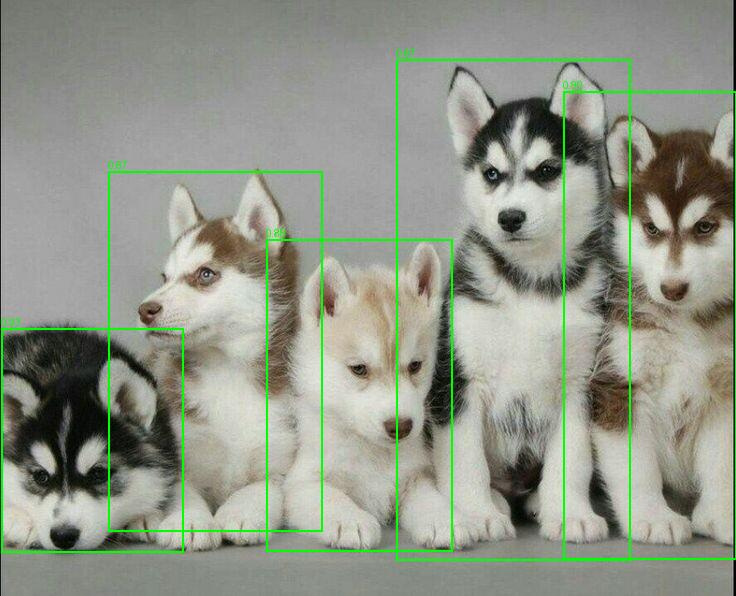
\includegraphics[width=\textwidth]{../results/figures/Yolov8s/husky_025.jpg}
\caption{YOLOv8s solo}
\end{subfigure}
\hfill
\begin{subfigure}{0.32\textwidth}
\includegraphics[width=\textwidth]{../results/figures/Yolov8s + Qwen0.8b/husky_025.jpg}
\caption{+ Qwen 0.8B}
\end{subfigure}
\hfill
\begin{subfigure}{0.32\textwidth}
\includegraphics[width=\textwidth]{../results/figures/Yolov8s + Qwen2.0b/husky_025.jpg}
\caption{+ Qwen 2B}
\end{subfigure}
\caption{Éxito claro (\texttt{husky\_025.jpg}): 5 cachorros en fila, todos detectados con cajas
ajustadas en las 3 configuraciones, sin falsos positivos ni falsos negativos.}
\label{fig:exito}
\end{figure}

\begin{figure}[H]
\centering
\begin{subfigure}{0.32\textwidth}
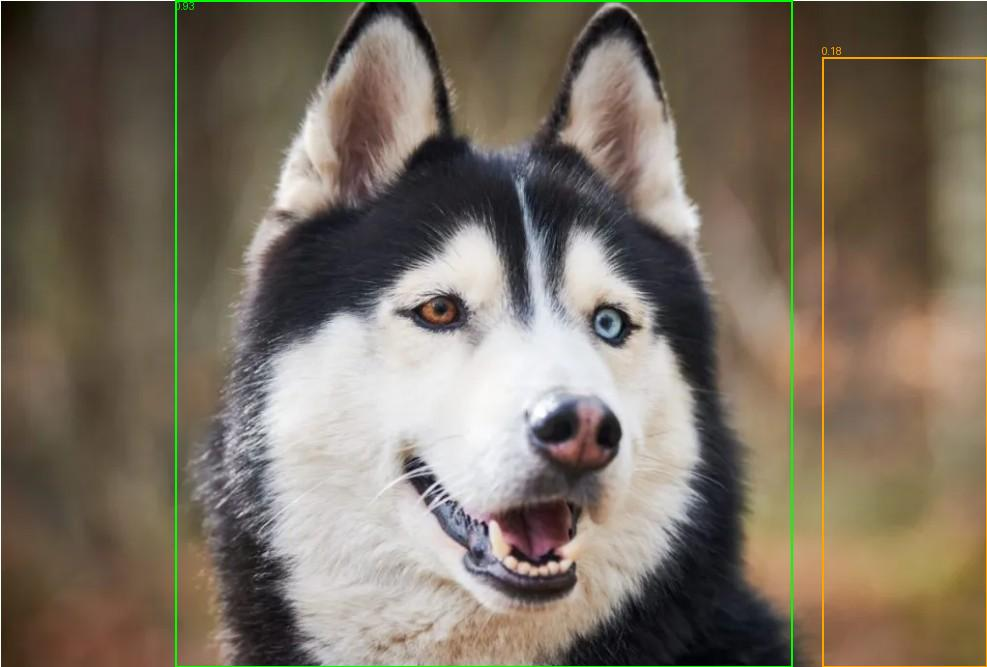
\includegraphics[width=\textwidth]{../results/figures/Yolov8s/husky_003.jpg}
\caption{YOLOv8s solo}
\end{subfigure}
\hfill
\begin{subfigure}{0.32\textwidth}
\includegraphics[width=\textwidth]{../results/figures/Yolov8s + Qwen0.8b/husky_003.jpg}
\caption{+ Qwen 0.8B}
\end{subfigure}
\hfill
\begin{subfigure}{0.32\textwidth}
\includegraphics[width=\textwidth]{../results/figures/Yolov8s + Qwen2.0b/husky_003.jpg}
\caption{+ Qwen 2B}
\end{subfigure}
\caption{Falso positivo mitigado por ambas versiones de la cascada (\texttt{husky\_003.jpg}):
YOLOv8s solo detecta correctamente al husky (conf.\ 0.93) pero también genera una caja espuria
sobre el fondo desenfocado (conf.\ 0.18, sin ningún perro dentro); tanto el validador de 0.8B
como el de 2B rechazan esa caja.}
\label{fig:fp-mitigado}
\end{figure}

\begin{figure}[H]
\centering
\begin{subfigure}{0.32\textwidth}
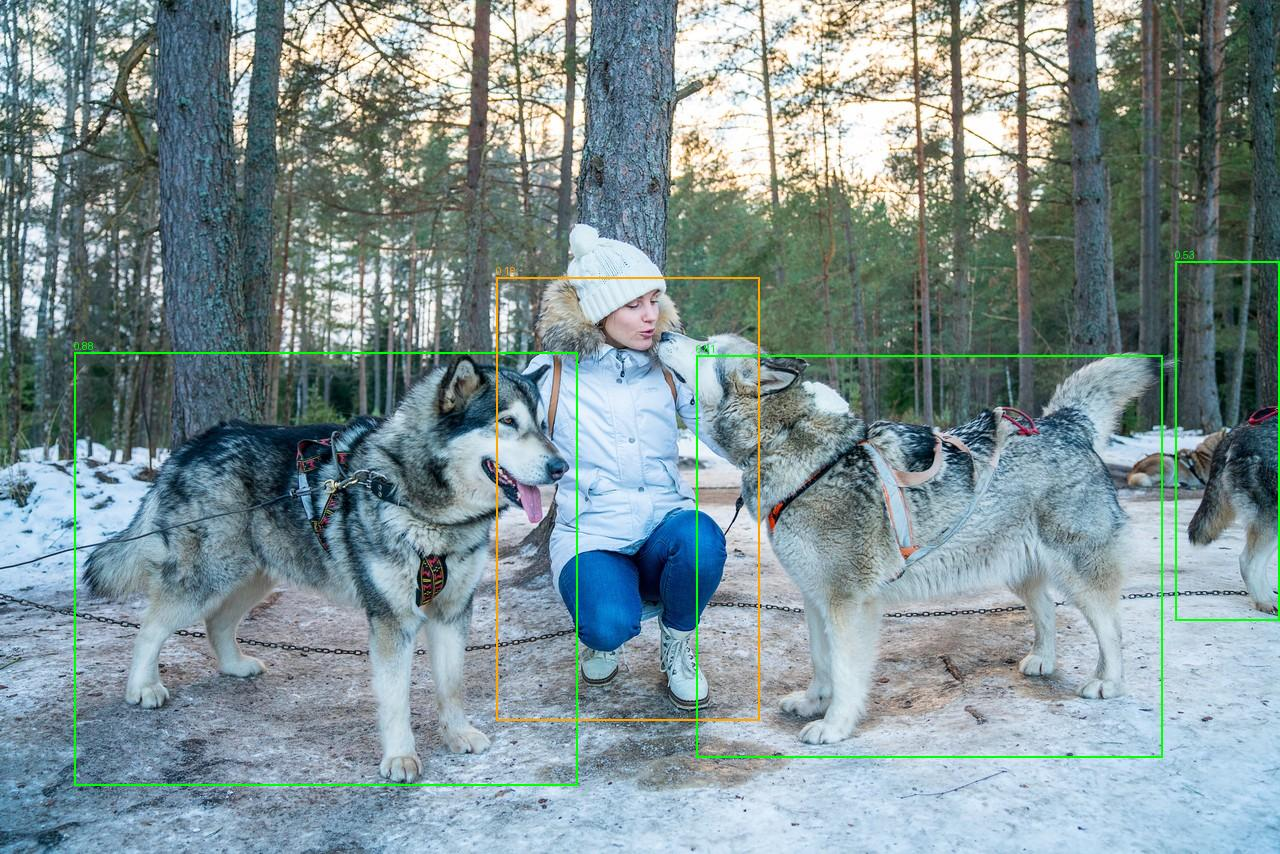
\includegraphics[width=\textwidth]{../results/figures/Yolov8s/husky_029.jpg}
\caption{YOLOv8s solo}
\end{subfigure}
\hfill
\begin{subfigure}{0.32\textwidth}
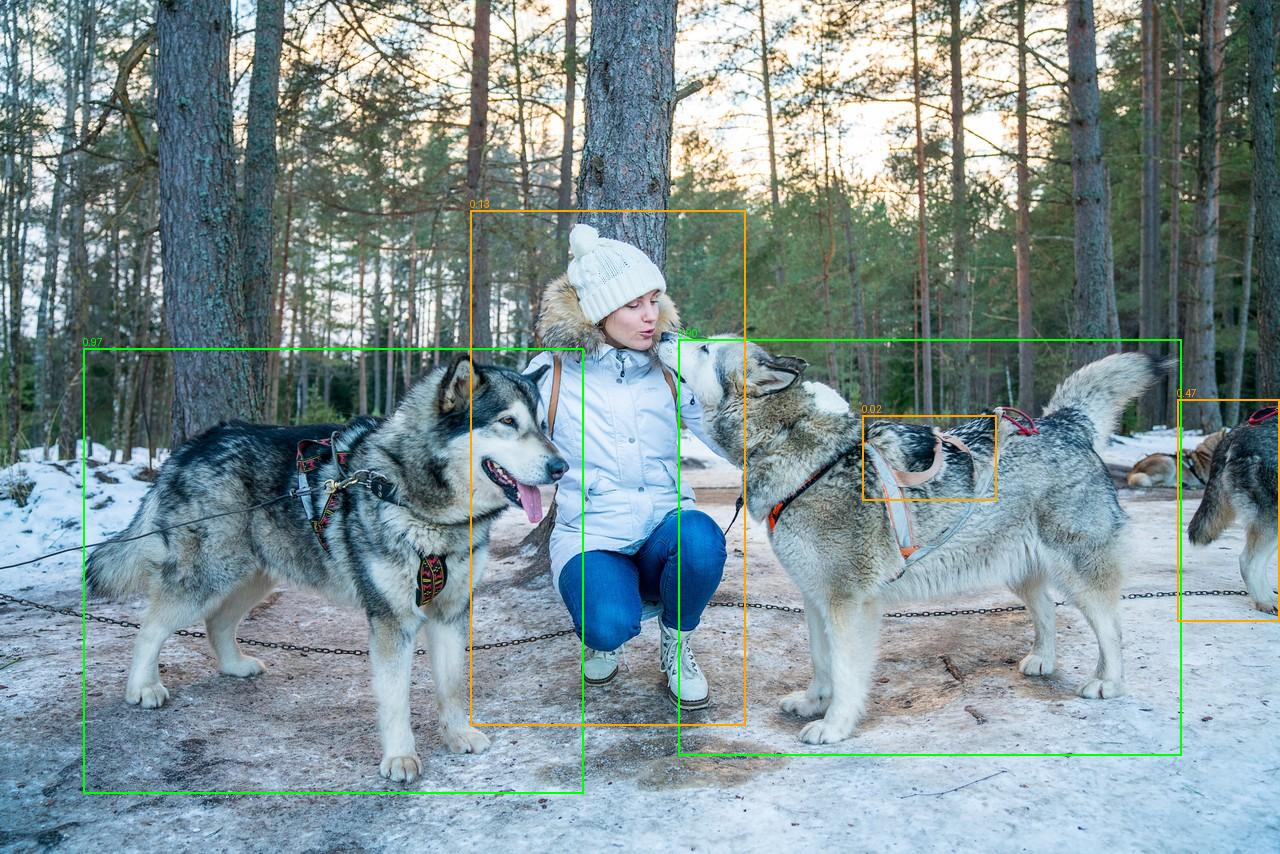
\includegraphics[width=\textwidth]{../results/figures/Yolov8s + Qwen0.8b/husky_029.jpg}
\caption{+ Qwen 0.8B}
\end{subfigure}
\hfill
\begin{subfigure}{0.32\textwidth}
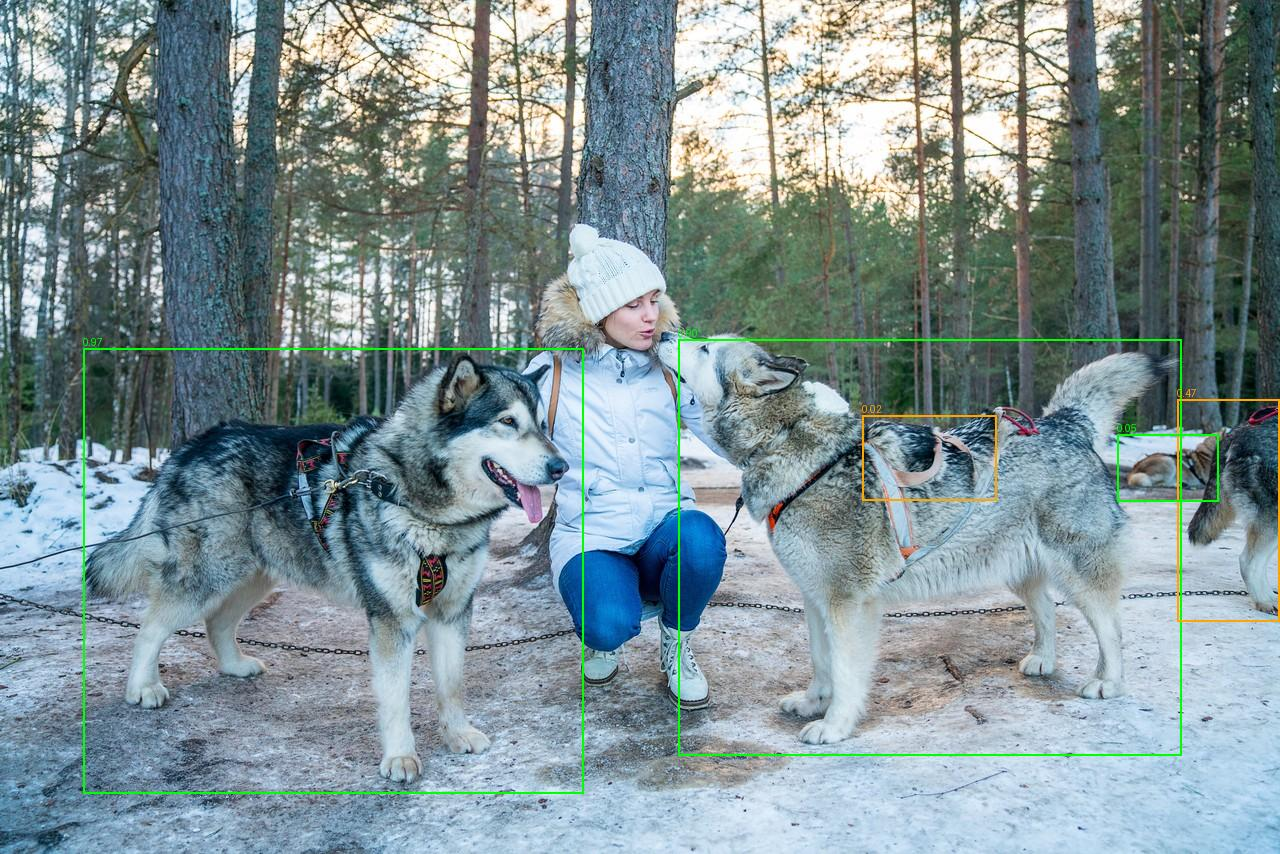
\includegraphics[width=\textwidth]{../results/figures/Yolov8s + Qwen2.0b/husky_029.jpg}
\caption{+ Qwen 2B}
\end{subfigure}
\caption{Caso de falla (\texttt{husky\_029.jpg}): imagen con varios perros, una persona en
primer plano y un perro adicional cortado por el borde derecho del encuadre. YOLOv8s solo
genera, además de las detecciones correctas, una caja falsa sobre la persona (conf.\ 0.13); el
validador de 2B la rechaza correctamente, pero el de 0.8B no. El perro parcialmente visible en
el borde derecho no recibe una confirmación sólida en ninguna de las 3 configuraciones.}
\label{fig:falla}
\end{figure}

% ============================================================
\section{Cuestionario de Análisis Crítico}
\label{sec:cuestionario}
% ============================================================

\subsection*{2. Penalización de recursos computacionales}

La activación de Qwen VL como validador en cascada degrada el FPS de forma drástica: de
\textbf{42.72 FPS} (YOLOv8s solo) a \textbf{0.45 FPS} con el validador de 0.8B y \textbf{0.43
FPS} con el de 2B en el conjunto de prueba, una caída superior a 90$\times$. Resulta notable que
la diferencia de tamaño entre 0.8B y 2B (2.5$\times$ más parámetros) prácticamente no se refleja
en el FPS (2198.84~ms vs.\ 2328.17~ms de latencia promedio, una diferencia menor al 6\,\%). Esto
indica que, para recortes pequeños de imagen y prompts binarios cortos, el cuello de botella no
es el cómputo asociado a los parámetros del modelo en sí, sino costos fijos por llamada (carga
de la imagen, \textit{overhead} de generación, \textit{tokenización}) que dominan sobre la
diferencia de tamaño del modelo.

Con estos números, el pipeline \textbf{no es viable} para un sistema de tiempo real crítico como
un vehículo autónomo, donde se requieren decenas de FPS con latencias de pocos milisegundos y
consecuencias de seguridad ante un retraso. A menos de 1 FPS, cada detección tarda más de 2
segundos en confirmarse, lo cual solo resulta aceptable en \textbf{aplicaciones asíncronas}
donde la latencia no es crítica: por ejemplo, etiquetado \textit{offline} de un archivo de
imágenes, un sistema de moderación de contenido que procesa una cola en segundo plano, o una
alerta de vigilancia que no necesita confirmarse en tiempo real. Para un caso de uso en tiempo
real, sería preferible usar solo YOLOv8s ($\sim$43 FPS) y aceptar la tasa de falsos positivos
considerablemente mayor, o explorar la alternativa de un clasificador ligero descrita en la
pregunta 5.

\subsection*{3. Propagación del error}

Un error sistemático de desalineación en las cajas generadas por el VLM durante la Fase~1 se
propaga directamente a la función de pérdida de regresión de YOLOv8s (\textit{Bounding Box
Loss}, compuesta por \textit{box\_loss}/CIoU y \textit{dfl\_loss} en la implementación de
Ultralytics). Si las cajas de \textit{ground truth} están sistemáticamente desplazadas o mal
dimensionadas (por ejemplo, consistentemente más anchas de lo real, o recortando extremidades
ocluidas), la red \emph{aprende ese sesgo como si fuera la verdad}: el optimizador ajusta los
pesos para minimizar la distancia a cajas que ya están mal ubicadas, por lo que el modelo
entrenado reproduce el mismo error sistemático en sus propias predicciones, en lugar de aprender
la localización real del objeto. Un error \emph{aleatorio} (ruido sin sesgo consistente)
tendería a promediarse y afectar menos al modelo; un error \emph{sistemático} (sesgo
direccional) degrada la precisión de localización de forma persistente, ya que no hay señal
contradictoria en los datos que lo corrija.

Un riesgo análogo puede darse no solo en la localización sino también en la \emph{clase}: si el
pseudo-\textit{ground truth} de la Fase~1 incluyera perros de otras razas visualmente similares
etiquetados como husky, ese sesgo se heredaría directamente en la evaluación posterior, sin que
el pipeline tenga forma de detectarlo por sí solo. Este riesgo motivó incorporar el paso de
verificación de raza descrito en la Sección~2.1.

\paragraph{¿Es necesario que un humano revise las anotaciones automáticas?} Sí. El auto-etiquetado
no es infalible, y el riesgo de sesgo sistemático de clase descrito arriba ilustra que este tipo
de error puede sobrevivir a una revisión automática si no se diseña específicamente para
detectarlo. El proyecto incorporó un paso de verificación visual de las anotaciones antes de
entrenar; un humano no necesita re-etiquetar todo el conjunto desde cero, pero sí debe hacer una
revisión de muestreo dirigida a detectar sesgos sistemáticos (no solo cajas mal ubicadas) antes
de que se propaguen al entrenamiento.

\subsection*{4. Sensibilidad del \textit{prompt engineering}}

El proyecto evaluó dos versiones del prompt de auto-etiquetado. La primera versión, más corta y
genérica (``Detect all husky dogs in this image. Return a JSON list...''), en ocasiones se
detenía tras detectar solo el primer perro de la imagen o variaba el formato de salida
(agregando texto explicativo o marcado de tipo \textit{markdown} alrededor del JSON), lo cual
dificultaba el parseo automático. La versión final, más larga y prescriptiva, que insiste
explícitamente en no detenerse tras la primera instancia, pide cajas ajustadas sin adivinar
partes ocluidas, y prohíbe explícitamente cualquier formato adicional, redujo notablemente esa
varianza. Esto confirma que Qwen3.5 es \textbf{sensible a la formulación exacta del prompt},
especialmente en instrucciones de completitud (``todas las instancias'') y de formato de salida
estricto: dejar espacio de interpretación se traduce directamente en inconsistencia en las
coordenadas y en fallas de parseo, no solo en la calidad semántica de la detección.

Sobre el prompt de validación binaria (Fase~4): funcionó de forma consistente y sin ambigüedad
para ambos tamaños de modelo en cuanto a formato (respuesta ``Yes''/``No'' bien formada en
prácticamente todos los casos). En cuanto a calibración, la Tabla~\ref{tab:comparativa-test}
muestra que el validador de 2B alcanza un mAP@0.5 ligeramente superior (0.9549 vs.\ 0.9376) y un
falso negativo menos que el de 0.8B, a costa de un falso positivo adicional (29 vs.\ 28): una
diferencia marginal que sugiere que, con el prompt final empleado, ambos tamaños de modelo
aplican un criterio de decisión comparable sobre las mismas instrucciones, sin que uno domine
claramente sobre el otro.

\subsection*{5. Optimización arquitectónica}

Reemplazar el validador VLM por un clasificador convolucional ligero entrenado desde cero (p.\
ej.\ ResNet18 o MobileNet) sobre los recortes de detección tiene un argumento de eficiencia
computacional muy fuerte a su favor: los datos de este mismo proyecto lo evidencian, ya que un
clasificador especializado y pequeño correría en el orden de milisegundos por recorte (similar a
la latencia de YOLOv8s, $\sim$23~ms para una imagen completa), frente a los $\sim$2.2--2.3
segundos por imagen que toma la cascada con Qwen VL en este pipeline. La ganancia de FPS
potencial es de varios órdenes de magnitud, precisamente lo que se necesitaría para acercarse a
un escenario de tiempo real (pregunta 2).

\paragraph{Ventajas del clasificador ligero.}
\begin{itemize}[nosep]
  \item Latencia y consumo de memoria órdenes de magnitud menores (millones de parámetros vs.\
  cientos de millones/miles de millones en Qwen).
  \item Al ser un modelo de clasificación binaria dedicado, puede optimizarse/cuantizarse
  agresivamente (INT8, TensorRT) sin la complejidad de un modelo generativo de lenguaje.
  \item No depende de que un LLM interprete correctamente un prompt en lenguaje natural: el
  espacio de salida es fijo, eliminando el riesgo de que el modelo produzca texto plausible pero
  incorrecto.
\end{itemize}

\paragraph{Desventajas del clasificador ligero frente al VLM.}
\begin{itemize}[nosep]
  \item Requiere un conjunto de entrenamiento etiquetado específico (recortes positivos/negativos
  de husky vs.\ no-husky) que en este proyecto no existe de forma independiente; habría que
  generarlo, posiblemente con el mismo VLM, reintroduciendo el problema original que motivó usar
  un VLM en primer lugar.
  \item Pierde la capacidad de razonamiento semántico general de un VLM: Qwen puede, en
  principio, generalizar mejor a variaciones no vistas en entrenamiento (ángulos, oclusiones,
  fondos inusuales) gracias a su preentrenamiento masivo, mientras que un CNN pequeño entrenado
  desde cero con pocos datos es más propenso a sobreajustarse a las particularidades del
  conjunto de entrenamiento.
  \item Menos flexible ante cambios de tarea: cambiar el criterio de validación en el VLM es
  solo cuestión de reescribir el prompt; en un clasificador dedicado requeriría reentrenar.
\end{itemize}

\paragraph{Conclusión.} Para un despliegue de producción con restricciones de tiempo real, un
clasificador ligero es la opción técnicamente más razonable, y sería el paso natural siguiente
si este proyecto continuara más allá del alcance académico actual. El uso de Qwen VL como
validador en este proyecto se justifica más bien por su propósito exploratorio/académico
(evaluar la viabilidad de un pipeline basado enteramente en un VLM, sin necesidad de generar un
conjunto de clasificación adicional) que por ser la opción óptima de producción.

% ============================================================
\section{Conclusiones}
% ============================================================

El pipeline implementado demuestra que es posible construir un detector de objetos
razonablemente preciso (mAP@0.5 $\approx 0.95$ en el conjunto de prueba, con la cascada de 2B)
partiendo de cero etiquetas manuales, usando un VLM abierto tanto para generar las anotaciones
de entrenamiento como para validar las detecciones en producción. La cascada de validación con
Qwen VL cumple su objetivo de reducir falsos positivos de forma contundente (más de la mitad en
el conjunto de prueba), pero a un costo de FPS que la hace inviable para aplicaciones de tiempo
real estricto, y su calibración no es perfectamente uniforme entre tamaños de modelo, como se
discute en la pregunta~4 del cuestionario.

Es importante señalar que las cifras de la Sección~\ref{sec:tabla-test} se obtuvieron sobre el
mismo conjunto de prueba empleado internamente por Ultralytics como conjunto de validación
durante el entrenamiento (Sección~\ref{sec:fase2}), por lo que conservan un ligero sesgo
optimista. Las demás limitaciones documentadas (pérdida de las clases de COCO originales, costo
computacional de la cascada) son conocidas y estarían mitigadas parcialmente por líneas de
trabajo futuro puntuales: preservar las clases de COCO mediante una segunda cabeza de detección,
mantener un conjunto de validación genuinamente separado del conjunto de prueba, y sustituir el
validador VLM por un clasificador ligero especializado para casos de uso en tiempo real.

\end{document}
